\chapter{Global Planner}
\label{chap:global}

The task of the global planner is to assemble a specified target polyomino $T$ given an initial configuration $g_{init}$.
The configuration-space is explored by executing local plans developed by the local planner from \autoref{chap:local}.
That way, the part of the configuration-space we can actually explore, is limited to configurations were a connection attempt between two cubes was made.
Compared to $SE(2)$ this part is manageable in size and only contains configurations which are interesting for self-assembly.

The question still remains, how these configurations are explored.
Using rapidly-exploring random trees (RRTs) \cite{lavalle1998} yields good results in a lot of cases, since the space gets evenly explored without the problematic of determining what decisions are promising for the end goal.
But, it also means the exploration of many configurations, which are not neccessary for reaching the goal.
For us this approach is not reasonable. 
Because of the high fidelity simulation we are working with, the computation time for a local plan is huge, so planning the assembly of $T$ with as less local plans as possible is the aim for our global planner.

We need to make well though-through connection decisions, that are valid for assembling $T$, meaning some sort of building plan for a polyomino is needed.
Creating a building sequences by removing one tile at a time from the target was done by Becker et al. \cite{Becker2020}.
However, this does not consider sub-assemblies, so all cubes that are not to be connected, have to stay separated at any time and occurring sub-assemblies would lead to immediate failure.

It is hard to prevent sub-assemblies, so our approach uses an enumeration of cutting a polyomino into two pieces (\autoref{sec:twocutting}), which will be used for generating a so called two-cut-sub-assembly graph (\autoref{sec:tcsa}).
In \autoref{sec:global_algo} that graph will be used as a building instruction along side the exploration of the configuration-space.
For this technique the number of cubes in the workspace is limited to the size of $T$.
A take on why is this done and why the problem becomes more complex when working with extra cubes, is done in \autoref{sec:more_cubes}.




\section{Two-Cutting Polyominoes}
\label{sec:twocutting}

% define two cut for us, talk about other definitions of two-cuts state difference
% take about monoton two cuts they ensure cave and hole free sub-polyominoes
% how do we calc. two cuts from starting connection
% how calc. all two-cuts for a polyomino
% FIGURE example graphic for two cuts monoton/non-monoton. possibilities for 3x3




\section{Two-Cut-Sub-Assembly Graph}
\label{sec:tcsa}

\begin{figure}
	\centering
	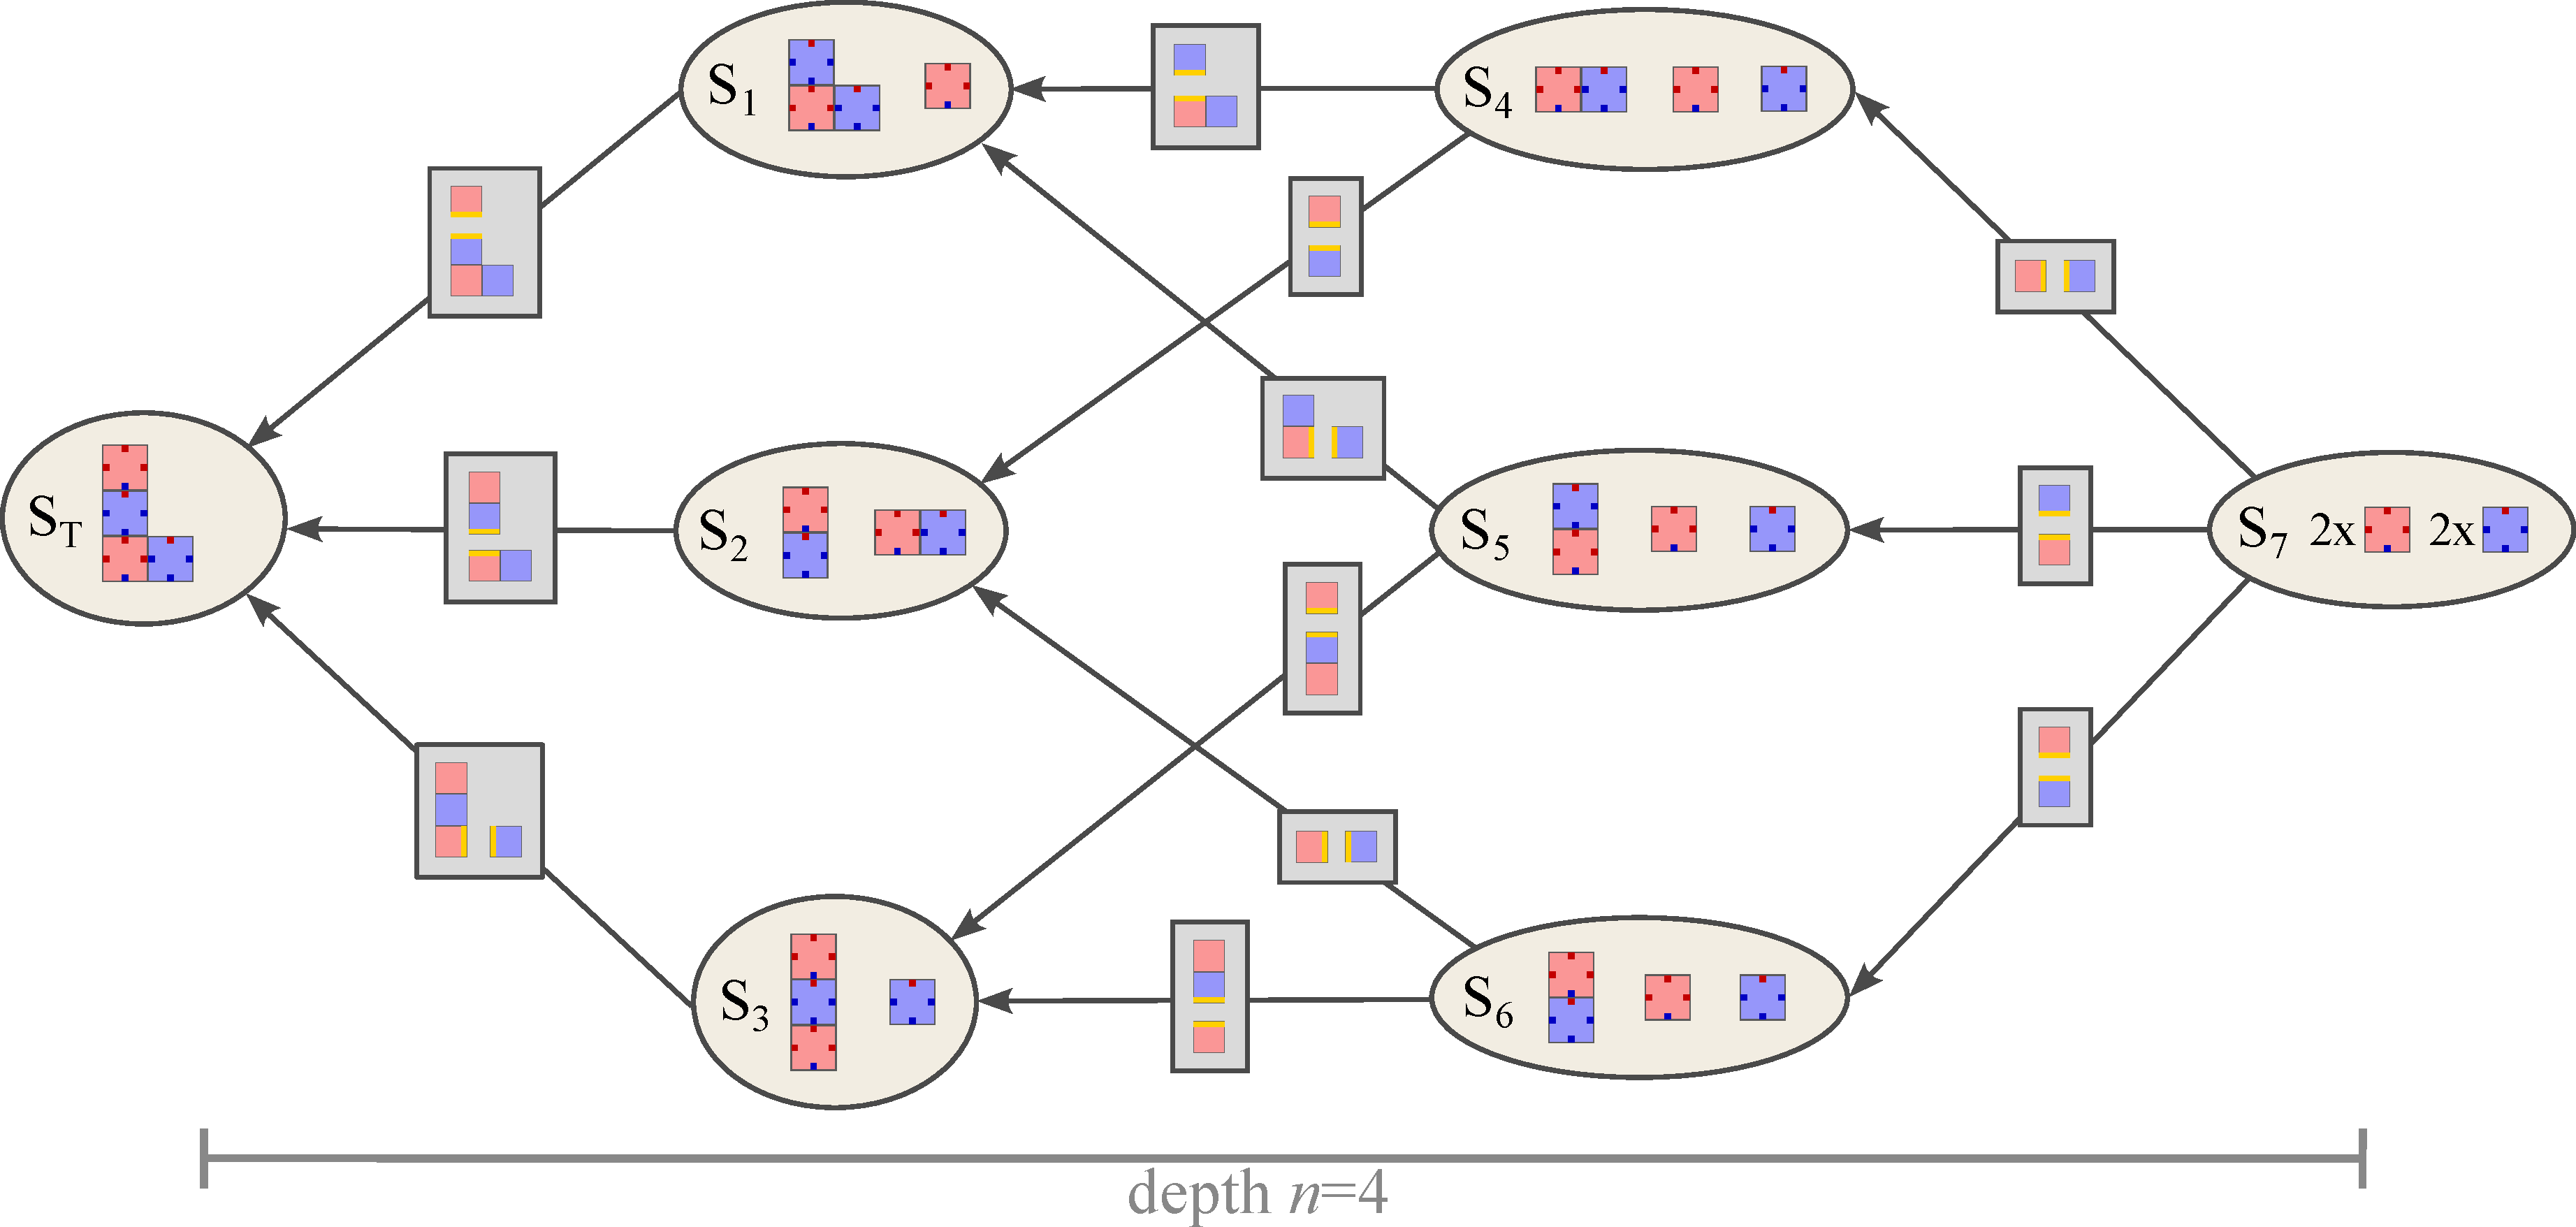
\includegraphics[width=1.00\textwidth]{figures/tcsa.pdf}
	\caption[Example for a two-cut-sub-assembly graph.]{long caption...}
	\label{fig:tcsa}
\end{figure}

% short TCSA-Graph
% purpes of this -> building sequence to target
% considering sets of polyominoes no positions in workspace
% notes are polysets edges connect polysets with (cube, cube, edge) conection as weigth. directiong from twocut to connected

\paragraph{Building TCSA-Graph}

% provide algorithm
% explain procedure with special cases
% - endup at all trivial
% - depth of graph n
% - common predecessor
% - multiple edges for same notes -> example FIGURE 3x1 + 1x1 = 4x1
% big example FIGURE of TCSA graph should include all special cases

\paragraph{Complexity}

% sterling numbers second kind as upper bound: find literatur
% connectivity cuts notes, monotonie cuts notes
% Access to graph in O(1) due to hash comparing.
% Creation complex but worth it -> minimize sim-time
% show practical data for tcsa-notes per size. Box-Whisker PLOT




\section{Global Planning Algorithm}
\label{sec:global_algo}

% provide algorith
% use of tcsa-graph
% limit number of cubes to target size
% check inclusion of poly set from config in tcsa-graph
% example early failure if initial is not in tcsa


\subsection{Connection Options}

% talk about options per note all edges to neighboring notes
% now consider position pairwise for all physical of poly types. example FIGURE
% taking a option with local planner
% - due to subassembly might not end in desired poly set
% - even local failure -> continue planning if poly set in graph
% - add allowed-poly failure to local planner to check this runtime
% - failure type that are not valid for further planning


\subsection{Option Sorting}

% there can be alot options
% we need smart decisions to pick best

\paragraph{Minimal Distance}

\paragraph{Grow Largest Component}
% this resembles one tile at a time with subassemblys still possible

\paragraph{Grow Smallest Component}



\subsection{Graph Traversal}

% DFS traversal. try to get to target as fast as possible
% Fall back if all options tried
% note that we not traverse tcsa graph we actually traverse configurations.
% When 2 configs with same polyset occure still try all options for both, because position differs

\paragraph{Complexity}

% best case 1 local plan. realistic best case n-1
% we are not limited by notes in tcsa, because n configs for 1 note
% for each note there is a constant number of options and depth smaller n-1.
% we wont run infinitly, but worst case is still bad. state example each note 50 options

\paragraph{Discretize Configurations}

% dont know if I wil actually implement, but talk about benefits or why not that neccessary




\section{More Cubes than Target}
\label{sec:more_cubes}

% bigger tcsa with multiple end notes
% same tcsa
% - no simple hash check. check for set inclusion
% - a poly set can be included in multiple tcsa-notes -> increasing options per config